\documentclass[10pt, a4paper]{amsart}
% \documentclass[10pt,showpacs,preprintnumbers,footinbib,amsmath,amssymb,aps,prl,twocolumn,groupedaddress,superscriptaddress,showkeys]{revtex4-1}
\usepackage[]{graphicx}
\usepackage[]{hyperref}
\usepackage[]{physics}
\usepackage[]{listings}
\usepackage[T1]{fontenc}
\usepackage{color}
\usepackage[ruled,vlined]{algorithm2e}

\usepackage{amsmath, amsfonts, amssymb}
\usepackage{listings}
\usepackage[]{subcaption}

\newcommand{\erfc}{\text{erfc}}

% Definition of code and how the code should look.
\usepackage{xcolor}
\definecolor{codegreen}{rgb}{0,0.6,0}
\definecolor{codegray}{rgb}{0.5,0.5,0.5}
\definecolor{codepurple}{rgb}{0.58,0,0.82}
\definecolor{backcolour}{rgb}{0.95,0.95,0.92}
\definecolor{mygreen}{rgb}{0,0.6,0}
\definecolor{mymauve}{rgb}{0.58,0,0.82}


\lstdefinestyle{python3}{
    backgroundcolor=\color{backcolour},
    commentstyle=\color{codegreen},
    keywordstyle=\color{magenta},
    numberstyle=\tiny\color{codegray},
    stringstyle=\color{codepurple},
    basicstyle=\ttfamily\footnotesize,
    breakatwhitespace=false,
    breaklines=true,
    captionpos=b,
    keepspaces=true,
    numbers=left,
    numbersep=5pt,
    showspaces=false,
    showstringspaces=false,
    showtabs=false,
    tabsize=2
}
% End def.



\lstset{ %
  backgroundcolor=\color{white},   % choose the background color; you must add \usepackage{color} or \usepackage{xcolor}
  basicstyle=\footnotesize,        % the size of the fonts that are used for the code
  breakatwhitespace=false,         % sets if automatic breaks should only happen at whitespace
  breaklines=true,                 % sets automatic line breaking
  captionpos=b,                    % sets the caption-position to bottom
  commentstyle=\color{mygreen},    % comment style
  deletekeywords={...},            % if you want to delete keywords from the given language
  escapeinside={\%*}{*)},          % if you want to add LaTeX within your code
  extendedchars=true,              % lets you use non-ASCII characters; for 8-bits encodings only, does not work with UTF-8
  frame=single,	                   % adds a frame around the code
  keepspaces=true,                 % keeps spaces in text, useful for keeping indentation of code (possibly needs columns=flexible)
  keywordstyle=\color{blue},       % keyword style
  language=python,                    % the language of the code
  style = python3,
  otherkeywords={*,...},           % if you want to add more keywords to the set
  rulecolor=\color{black},         % if not set, the frame-color may be changed on line-breaks within not-black text (e.g. comments (green here))
  showspaces=false,                % show spaces everywhere adding particular underscores; it overrides 'showstringspaces'
  showstringspaces=false,          % underline spaces within strings only
  showtabs=false,                  % show tabs within strings adding particular underscores
  stepnumber=2,                    % the step between two line-numbers. If it's 1, each line will be numbered
  stringstyle=\color{mymauve},     % string literal style
  tabsize=2,	                     % sets default tabsize to 2 spaces
}

\title[Problem set 3]{Problem set 3: Dissusion and Advection\\
\normalsize{Due: 3 Nov. 2020} \\
  \hrulefill\small{GEO2300: Fysiske prosesser i geofag }\hrulefill}

\author[Sundberg]{Sigurd Sandvoll Sundberg}
\date{\today}

\begin{document}
\maketitle

\section{Problem 1: The Diffusive Climate Model.}
We want to consider a diffusive climate model, where we will divide the earth into small slices along the latitude lines. Each section is $1^\circ$ tall, and goes around the entire Earth. We essentially slice the Earth like an apple, in small slices, and assume that the temperature in each slice is the same. 
\subsection{a)}
Starting of with a simple climate model discussed in the compendium\cite{joe}, and expanding it with a diffusive term, so our governing equation is 
\begin{equation}\label{eq:a}
	\frac{\partial}{\partial t}T = \frac{1}{\rho c_pH} \left(\frac{S}{4}\left(1-\alpha\right) - \epsilon\sigma T^4\right) + \frac{D}{R_E^2}\frac{\partial^2}{\partial \theta^2}T
\end{equation}
where we have the following constants
\begin{itemize}
	\item $\rho = 1\,[kg/m^3]$,
	\item $c_p = 1004\,[J/(K\,kg)]$,
	\item $H = 10^4\,m$,
	\item $S/4 = 350\cos(\theta) + 150 \,[W/m^2]$,
	\item $\alpha = 0.7 - 0.45\cos(\theta)\, [-]$,
	\item $\sigma = 5.67 \times 10^{-8}\, [W/(m^2K)]$,
	\item $\epsilon = 0.6\, [-]$,
	\item $R_E = 6.37\times 10^6\,[m]$,
	\item $d\theta = \pi/180$.
\end{itemize}

Writing out equation \ref{eq:a}, using the FTCS scheme we have 
\begin{align}
	\frac{T_j^{n+1}- T_j^n}{dt} &= \frac{1}{\rho c_pH}\left(\frac{S_j}{4}\left(1-\alpha\right) - \epsilon\sigma \left(T_j^n\right)^4\right) + \frac{D}{R_E^2}\left(\frac{T^n_{j+1}-2T_j^n + T_j^n}{d\theta^2}\right)\\
	T_j^{n+1} &= \frac{dt}{\rho c_pH}\left(\frac{S_j}{4}\left(1-\alpha\right)\right) - \frac{\epsilon\sigma dt}{\rho c_pH} \left(T_j^n\right)^4 + \frac{Ddt}{R_E^2d\theta^2}\left(T^n_{j+1}-2T_j^n + T_j^n\right) + T_j^n && \text{$s = (dt D)/(R_E^2d\theta^2)$}\\
	T_j^{n+1} &= sT_{j+1}^n +(1- 2s)T_j^n + sT_{j-1}^n + \frac{dt}{\rho c_pH}\left(\frac{S_j}{4}\left(1-\alpha\right)\right) - \frac{\epsilon\sigma dt}{\rho c_pH} \left(T_j^n\right)^4\label{eq:A}
\end{align}
which can be rewritten on the follow form 
\begin{equation}
	T^{n+1} = \mathbf{A}T^n + F
\end{equation}
where we have 
\begin{equation}
	F = q_1\left(\frac{S_j}{4}\left(1-\alpha\right)\right) - q_2\left(T_j^n\right)^4
\end{equation}
with $q_1 = \frac{dt}{\rho c_pH}$ and $q_2 = \frac{\epsilon\sigma dt}{\rho c_pH} $.

Matrix $\mathbf{A}$ is given by the following terms 
\begin{equation}
	sT_{j+1}^n +(1- 2)T_j^n + sT_{j-1}^n.
\end{equation}

Using that we have no flux at the poles, we have Neumann boundary conditions given by 
\begin{equation}
	\frac{\partial}{\partial \theta} T = 0, \quad T_0 = T_{-1} \land T_{n+1} = T_n
\end{equation}
Studying the boundaries of our problem we have the following
\begin{align}
	T_0 &= sT_1 + (1-2s)T_0 + sT_0 = sT_1 + (1-s)T_0\\
	&\vdots \\
	T_n &= sT_n + (1-2s)T_n + sT_{n-1} = (1-s)T_n + sT_{n-1}
\end{align}
Our matrix $\mathbf{A}$ then looks as follows 
\begin{equation}
	\mathbf{A} = 
	\begin{bmatrix}
		1 - s & s & 0 & \dots & \dots \\
		s & 1-2s & s & 0 & \dots \\
		\dots & \dots & \dots & \dots & \dots \\
		\dots & 0 & s & 1-2s & s \\
		\dots & \dots & 0 & s & 1-s \\
	\end{bmatrix}\label{mat:A}
\end{equation}

Converting the FTCS scheme to Python code, could result in the following script
\lstinputlisting[firstline=16, lastline=114]{../code/1a.py}
Imports and plotting labels are left out.

Studying a model where we use different values for D, namely $D = \lbrace1\times 10^6, 5\times 10^6, 1\times 10^7, 5\times 10^7,\rbrace[m^2/s]$ and compare our results against the case without diffusivity, where we choose dt such that $s = 0.4$ and use a final time of 10 times $T_{\text{rad}} = 140$days\cite{joe} to achieve a steady state solution. 
Seen in figure \ref{fig:1a} we have the four cases with increasing diffusivity, where the steady state solutions minimum and maximum value, gets closer the higher diffusivity becomes. This means that the temperature at the poles would be closer to that of the equator the higher diffusivity becomes. 

Whilst in the zero diffusivity case, we have large difference in temperature between the poles and equator, in the highest diffusivity case we have almost the same temperature at the poles as we do at equator. 
\begin{figure}
	\centering
	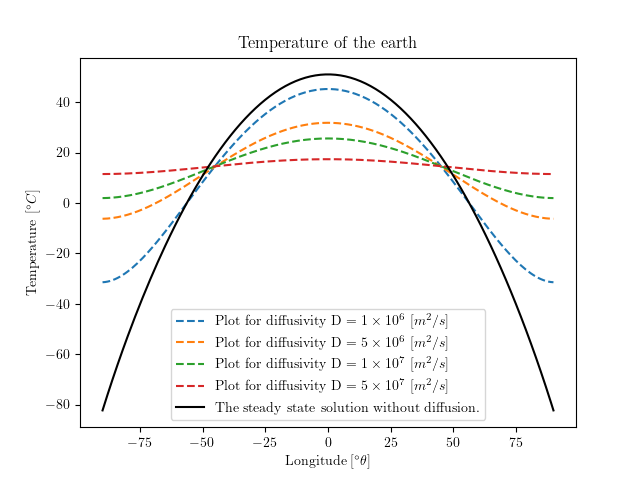
\includegraphics[width=0.9\textwidth]{../code/Figure_1.png}
	\caption{The case with no diffusivity, plotted against cases with diffusivity. Along the y-axis the temperature is shown and along the x-axis, longitude is shown. On the edges of the plot, we have the north and the south pole, whilst in the middle is the equator. Seen is that as diffusivity increases the difference between cold and warm areas diminish, and if diffusivity becomes high enough, there would be no visible difference.}
	\label{fig:1a}
\end{figure}

\subsection{b)}
Considering different climate model where we look at how changes in the emissivity $\epsilon$ of the atmosphere changes the global temperature. As a baseline case we will use the diffusive climate model with $D = 10^7$ m/s. We want to find out how much we would need to change the emissivity to achieve a global average temperature increase of $5^\circ$ Celsius. 

We can adapt our program from part a), with only adding the following small modifications 
\lstinputlisting[firstline=92, lastline=123]{../code/1b.py}

The rest of the function definitions are the same as for the a), only modifications the main part of the script was needed to adapt our code. 

From this we can extract the following results
\begin{lstlisting}
	To achieve a 5 degree average temperature change the emmisivity needs to be: 0.560
	The difference in maximum and minimum tempratures is 0.099
\end{lstlisting}
From which we can see, that to achieve a global warming of $5^\circ$ Celsius, we would need to change the emissivity from $0.58$ to $0.56$. Also we have that the difference between the minimum and maximum values of the difference between the case with 0.58 and 0.56 emissivity, is only $0.1^\circ$ Celsius. This is supported by figure \ref{fig:1b}, where we see a minimal difference between the equator and the poles. So we can fairly confidently that the increase in global temperature follows a uniform increase.
\begin{figure}
	\centering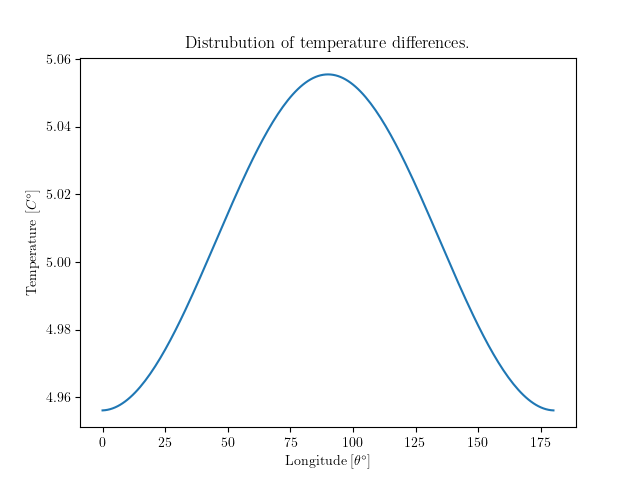
\includegraphics[width=0.9\textwidth]{../code/1b.png}
	\caption{Difference between the emissivity 0.58 and 0.56 in degrees Celsius. We see that the transform seems fairly uniform, with minimal difference between the edges. It has the same shape as our non-diffusivity case, and represents a large increase, though minimal, at the equator compared to the poles.}
	\label{fig:1b}
\end{figure}
\subsection{c)}
Going back to the diffusive climate model with emissivity $0.58$, we want to study what a change in the albedo would result in. We will consider a case where the ice on the poles disappeared in the future, and see how this change would affect the global climate. Firstly the ice on the north pole, would result in more open water being visible to the Sun, and water has a low albedo. For the south pole we would have visible land which again have a higher albedo than ice. 

We will adapt the albedo, to represent this, however not with accurate values. We will still use a small difference in albedo between the poles and equator, but much lower than our base case. From figure \ref{fig:1c1}, we see the changed albedo, and see how much the temperature increase when we change the albedo. This is due to the angle at which the light hits the Earth surface at the poles compared to the equator, at a higher angle more light will be reflected, thus the albedo should be higher at the poles even without ice. 
Even though we have the same albedo at the equator, we see a large increase in the equator temperature. This comes from the fact that diffusivity tries to average the global temperature, and as it is warmer at the poles, we would have less warm air would need to move from the equator to the poles to average the global temperature. We can see the change in temperature compared to our base case in figure \ref{fig:1c2}, which resembles the non-diffusivity case for our climate model. We see that increase in temperature is greatest at the pole due to a large change in the albedo. 

\begin{figure}
	\centering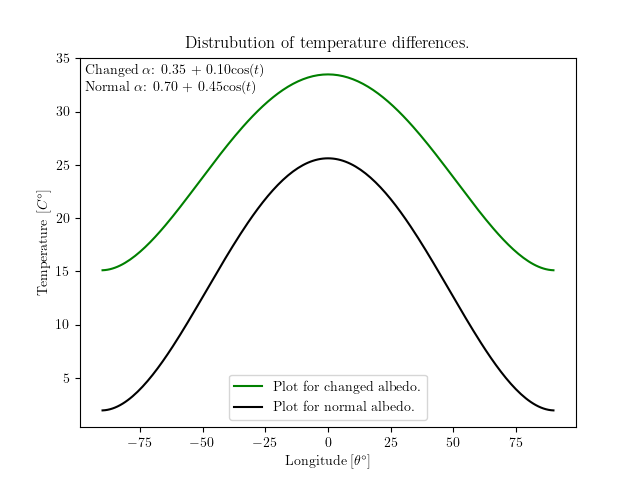
\includegraphics[width=0.9\textwidth]{../code/c1.png}
	\caption{The base case, plotted against a case where we have less ice on the poles. Values are not accurate representation of actual albedo that would come from poles without ice, however this represents a case where the albedo at equator is the same, and less at the poles.}
	\label{fig:1c1}
\end{figure}

\begin{figure}
	\centering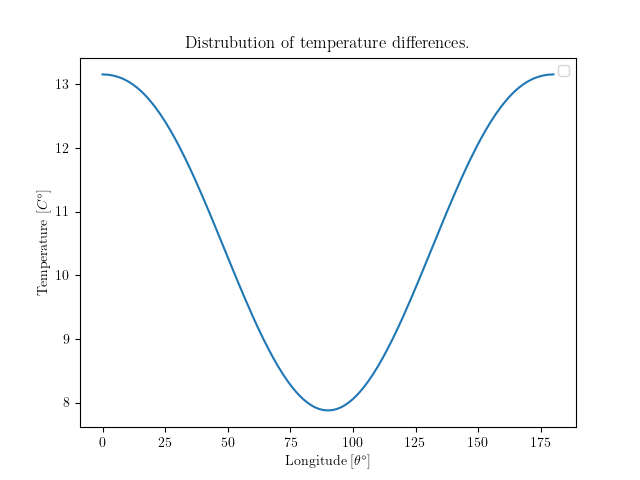
\includegraphics[width=0.9\textwidth]{../code/c2.png}
	\caption{The change in temperature from the base case. We see a large increase in temperature at the poles and a smaller one at the equator. This is resembles the inverse of the non-diffusivity case for our climate model.}
	\label{fig:1c2}
\end{figure}

We can again reuse the same code as in a) with the following changes 
\lstinputlisting[firstline=90, lastline=124]{../code/1c.py}

From this we get that the difference between the maximum and minimum values of the global temperature change is 
\begin{lstlisting}
	The difference in maximum and minimum tempratures is 5.278
\end{lstlisting}
from figure \ref{fig:1c2}. In other words the temperature at the poles increase by roughly 5 degrees Celsius more at the poles compared to the equator. 

\subsection{d)}
Another way we could study this climate model is to look at how a different numerical method reproduces the results. Or looking at stability of two different algorithms, perform when we change the variable $s = (dt D)/(R_E^2d\theta^2)$, which dictates our chosen value for dt. 

The Crank-Nicholson(CN) scheme, is a combination FTCS scheme, and its implicit version iFTCS. The iFTCS scheme looks as follows 
\begin{equation}
		- sT_{j+1}^{n+1} + (1 + 2s)T_j^{n+1} - sT_{j-1}^{n+1} = \\
		\\
		\frac{dt}{\rho c_pH}\left(\frac{S_j}{4}\left(1-\alpha\right)\right) - \frac{\epsilon\sigma dt}{\rho c_pH} \left(T_j^n\right)^4
\end{equation}
keeping our forcing terms from equation \ref{eq:A} the same, thus only changing the diffusivity terms. This is due to us having no good way of representing $(T^{n+1})^4$. 

Our CN scheme then becomes 
\begin{equation}
	- \frac{s}{2}T_{j+1}^{n+1} + (1 + s)T_j^{n+1} - \frac{s}{2}T_{j-1}^{n+1} = - \frac{s}{2}T_{j+1}^{n+1} + (1 - s)T_j^{n+1} + \frac{s}{2}T_{j-1}^{n} +\frac{dt}{\rho c_pH}\left(\frac{S_j}{4}\left(1-\alpha\right)\right) - \frac{\epsilon\sigma dt}{\rho c_pH} \left(T_j^n\right)^4
\end{equation}
which we can rewrite to 
\begin{equation}
	\mathbf{B}T^{n+1} = \mathbf{A}T^n + F
\end{equation}
where we define $\mathbf{A}$ and $\mathbf{B}$ the same as in equation \ref{mat:A}. 

Studying the boundary conditions of our problem which are the same as earlier, we have 
\begin{align}
	-\frac{s}{2}T_1^{n+1} + (1+s)T_0^{n+1} - \frac{s}{2}T_0^{n+1} &= sT_1^n + (1-s)T_0^n - sT_0^n \\
	\longrightarrow -\frac{s}{2}T_1^{n+1} + (1+\frac{s}{2})T_0^{n+1}&= sT_1^n + (1-\frac{s}{2})T_0^n\\
	&\vdots \\
	-\frac{s}{2}T_{j+1}^{n+1} + (1+s)T_j^{n+1} - \frac{s}{2}T_{j-1}^{n+1} &= sT_{j+1}^n + (1-s)T_{j}^n - sT_{j-1}^n \\
	\longrightarrow (1+\frac{s}{2})T_j^{n+1}-\frac{s}{2}T_{j-1}^{n+1} &=  (1-\frac{s}{2})T_{j}^n + sT_{j-1}^n
\end{align}

To implement the CN scheme, we can reuse almost all parts of our code in a), except we would need to define matrix $\mathbf{B}$ and redefine matrix $\mathbf{A}$ and find the matrix $B^{-1}A$ to solve $T^{n+1} = \mathbf{B}^{-1}\mathbf{A}T^n + F$. 

The changes needed are then a new setup for the CN scheme. Below are the two added functions and we run the program for s = 4 and s = 0.4. As usual plotting is left out. 
\lstinputlisting[firstline=53, lastline=74]{../code/1e.py}
\lstinputlisting[firstline=90, lastline=100]{../code/1e.py}
And the solver for FTCS and CN are called as follow
\begin{lstlisting}
	T_ftcs = solverFTCS(s, n, rho, epsilon, t_end, Sj, aj, dt)
	
	T_cn = solverCN(s, n, rho, epsilon, t_end, Sj, aj, dt)
\end{lstlisting}

Studying the results of this, we seen in figure \ref{fig:1e1} that there is no visible difference between the CN and FTCS schemes for s = 0.4. Meaning that for certain choices of s, for the FTCS this would be an s < 0.5, we can choose either scheme, and they would produce almost equal solutions. So as long as the FTCS scheme is stable, it is the preferred method as it is simpler to setup. 

When we look at s = 4, we can see from figure \ref{fig:1e2} that, for either value of s, the CN scheme, produces solution with no visible difference. That means that we can choose a large value for s, for which the FTCS scheme is not stable, and in turn have to do fewer iterations, to achieve the same result. Now iterations does not speak for total run time as the number of floating point operations are also needed to be taken into account. Mainly for constructing the matrices here, however this is beneficial either way. So for long term simulations, using the CN scheme, outperforms the FTCS scheme, as fewer iterations are required for the same results. 

Also to keep in mind, when trying our specific case for s = 4, using the FTCS scheme, we end up with a run time warning due to an overflow. Meaning that the FTCS scheme is blowing up and causing overflows for numerical values. This is not desirable, and we need to swap scheme, as we saw, the CN scheme performs perfectly here. This can also be seen from the Neumann stability analysis\cite{lev02}, where s < 0.5, for FTCS to be stable.


\begin{figure}
	\centering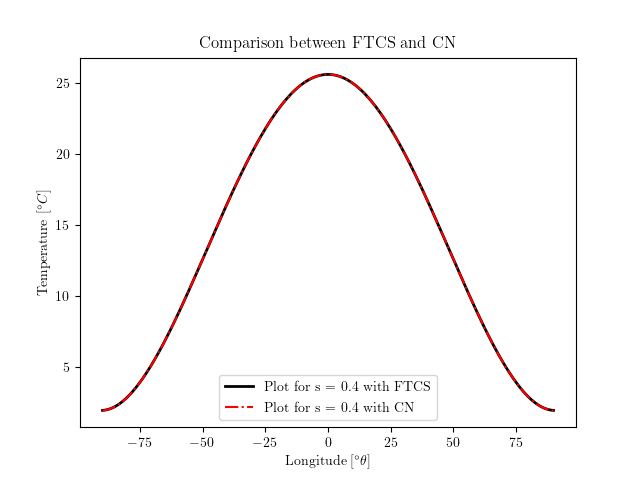
\includegraphics[width=0.9\textwidth]{../code/1e1.png}
	\caption{The FTCS scheme compared to CN scheme, plotting for s = 0.4. We see that the two scheme produces solutions which are visibly no different from each other. Both scheme seem stable, and have little to no variance. }
	\label{fig:1e1}
\end{figure}

\begin{figure}
	\centering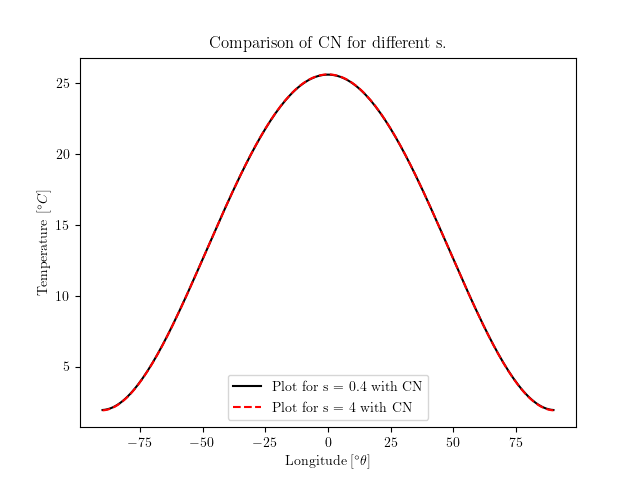
\includegraphics[width=0.9\textwidth]{../code/1e2.png}
	\caption{The CN scheme compared to itself for s = 4 and s = 0.4. We have no visible difference between the two choices of s.}
	\label{fig:1e2}
\end{figure}
\newpage
\subsection{e)}

\section{Problem 2: Woman Overboard, Without and With Eddies.}
We want to study how a body moves after falling into a river with and without eddies. We will look at this as a probability problem where we look at the probability of finding the person at position $x$ at time $t$ after initially falling into the river.

\subsection{a)}
What we know initially is that the woman, falls into the river about 100 m downstream from a dam. We are not sure exactly where she falls into the water, but know it is an area with a radius of 10 m. We assume the river flows at a constant velocity of 50 cm/s. 

To find the probability of where she fell into the river, we will describe the probability density function(PDF) as a Gaussian function. Thus it takes on the form 
\begin{equation}
	p(x) = \frac{1}{\sigma\sqrt{2\pi}}\exp\left(-\frac{(x-\mu)^2}{2\sigma^2}\right)
\end{equation}
where $\sigma$ is the standard deviation of 10 m and $\mu$ is the mean value of 100 m at $t=0$. Inserting these values we get the equation of the probability to find the woman at $t=0$, given any position $x$. This equation reads
\begin{equation}\label{PDF_i}
	p(x) = \frac{1}{10\sqrt{2\pi}}\exp\left(-\frac{(x-100)^2}{200}\right). 
\end{equation}

\subsection{b)}
As we are currently considering a case where we do not have any eddies in the river, the motion of the woman is only described by the advection due to the water flow. 

The general advection equation reads 
\begin{equation}\label{eq:ad}
	\frac{\partial}{\partial t}\phi + u\frac{\partial}{\partial x}\phi = 0
\end{equation}
where $\phi$ describes the property we are studying, in this case the probability of finding a woman in the river, and $u$ is the velocity of the river as we are only considering a one dimensional case. 

Using the method of characteristics, we know a given solution to equation \ref{eq:ad} can be expressed at $f(x-ut)$, where x is the position, u is the velocity and t is the time step. Applying this to equation \ref*{PDF_i}, we find that the analytical expression for the womans positions in time is given by 
\begin{equation}
	p(x-ut) = \frac{1}{10\sqrt{2\pi}}\exp\left(-\frac{(x-u*t - 100)^2}{200}\right),
\end{equation}
inserted for $u = 0.5$m/s we find 
\begin{equation}\label{eq:P}
	p(x-ut) = \frac{1}{10\sqrt{2\pi}}\exp\left(-\frac{(x-0.5*t - 100)^2}{200}\right). 
\end{equation}
which describes the probability to find the woman at position x at time t from the initial state.  

\subsection{c)}
We are interested in studying this problem numerically through expanding the advection equation, from a continuous problem to a discretized problem which we can evaluate numerically. 

Starting with the simplest numerical scheme, we consider the forward in time, centered in space(FTCS) scheme. Writing our the advection equation, using $p$ instead of $\phi$, we have 
\begin{align}
	\frac{\partial }{\partial t}p + u\frac{\partial}{\partial x}p &= 0\\
	\frac{p_i^{n+1}-p_i^n}{\Delta t} + u\frac{p_{i+1}^n - p_{i-1}^n}{2\Delta x} &= 0\\
	\frac{p_i^{n+1}-p_i^n}{\Delta t} &= -u\frac{p_{i+1}^n - p_{i-1}^n}{2\Delta x}\\
	p_i^{n+1} &= -u\Delta t\frac{p_{i+1}^n - p_{i-1}^n}{2\Delta x} +p_i^n\\	
	p_i^{n+1} &= -\frac{C_0}{2}\left(p_{i+1}^n - p_{i-1}^n\right) + p_i^n\label{eq:disc}
\end{align}
$p_i^n$, references the $i-$th index and $n-$th time step and $C_0 = (u\Delta t) / \Delta x$.

From equation \ref{eq:disc} we see that our problem takes on the form of 
\begin{equation}\label{eq:FTCS}
	p^{n+1} = \mathbf{P}p^n.
\end{equation}
Where $\mathbf{P}$ describes the matrix on the form 
\begin{equation}\label{mat:FTCS}
	\mathbf{P} = 
	\begin{bmatrix}
		1 & -C_0/2 & 0 & \dots & \dots\\
		C_0/2 & 1& -C_0/2 & 0 & \dots \\
		\dots & \dots & \dots & \dots &  \dots \\
		\dots & 0 & C_0/2 & 1 &  -C_0/2 \\
		\dots &  \dots & 0 & C_0/2 & 1
	\end{bmatrix}
\end{equation}
using Dirichlet boundary conditions $p_0 = 0 \land p_n = 0$. This is a safe assumption to make as the probability of finding the woman at the dam would be zero\footnote{She would essentially be found already as she would be on the dam.}, and can consider that at the end of the considered domain, there is something that causes the chance of finding the woman to be zero, such as a waterfall, pipe or similar. 

A Python script that creates the matrix $\mathbf{P}$ and plots the numerical against the analytical solution with the following parameters
\begin{itemize}
	\item $x\in [0,1000]$m
	\item dx = 5
	\item $\mu = 100$m
	\item $C = 0.1$
	\item u = 0.5m/s
	\item $\sigma = 100$m
	\item dt = (cdx)/u
	\item $t = [0,500,1000,1500]$s
\end{itemize}
can look as follows 
\lstinputlisting[firstline=11, lastline=63]{../code/2c.py}
excluded from the code is imports and extra plotting details for labels ect. 

\begin{figure}
	\centering
	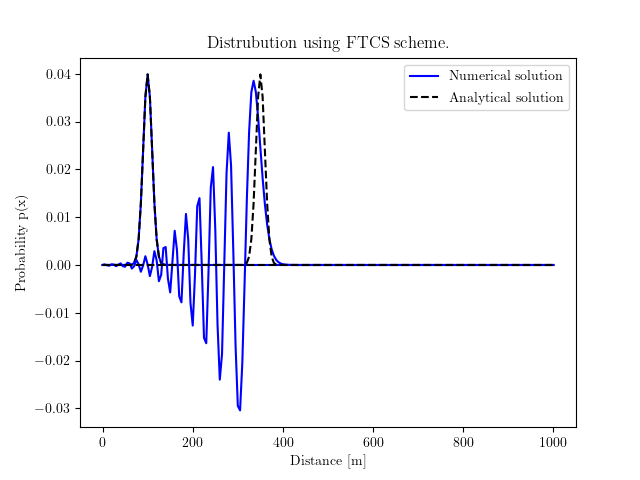
\includegraphics[width=0.9\textwidth]{../code/2c1.png}
	\caption{Plot of the FTCS scheme using t = 0 and t = 500. Already for t = 500, the numerical values are highly unstable and produces no usable results.}
	\label{fig:2c1}
\end{figure}

\begin{figure}
	\centering
	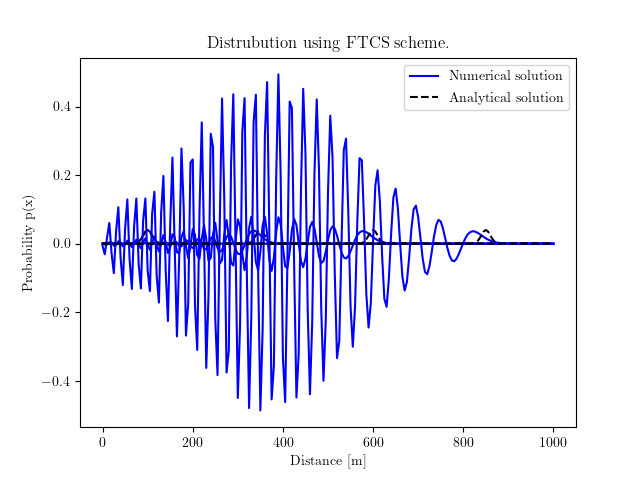
\includegraphics[width=0.9\textwidth]{../code/2c2.png}
	\caption{Plot using FTCS scheme, of the probability against position for different time steps. We see that the solution is extremely unstable, and produces no usable result. This goes for all values of t.}
		\label{fig:2c2}
\end{figure}

From figure \ref{fig:2c1} we see the plot for the value of t = 500s, which already produces an unstable solution. We can not use this data for anything, and this persists when we increase the final time as seen in figure \ref{fig:2c2}. Doing a stability analysis of the problem, we find that measure of stability, mainly $r = max\lbrace u\rbrace \cdot dt / dx$, for the FTCS scheme, is given by 
\begin{lstlisting}
	"Stability r: 0.020"
\end{lstlisting}
which for the FTCS scheme is should be stable. However applying the FTCS scheme to a one dimensional advection equation can be shown to be unconditionally unstable, thus we are presented with results which are unstable. This originates from the Von Neumann stability analysis of finite difference schemes\cite{lev02}. 

As we now know, we are unable to produce usable results with the FTCS scheme, instead let us consider the implicit forward in time, centered in space(iFTCS) scheme.  

\subsection{d)}
For the iFTCS scheme, we look at where we want to go, to decide where we are going, instead of looking at where we are to decide where we go. That means instead of solving equation \ref{eq:FTCS}, we are interested in solving 
\begin{equation}
	\mathbf{P}p^{n+1} = p^n\, \longrightarrow\, p^{n+1} = \mathbf{P}^{-1}p^n
\end{equation}
where $\mathbf{P}$ is defined to be the matrix originating from the following equation 
\begin{equation}
	\frac{C_0}{2}\left(p_{i+1}^{n+1}-p_{i-1}^{n+1}\right) + p_i^{n+1}= p^n
\end{equation}
created in the same way as \ref{mat:FTCS}.

The only changed needed to our code is how we define our matrix $\mathbf{P}$, the following function implements matrix $\mathbf{P}$ for the iFTCS scheme.
\lstinputlisting[firstline=26, lastline=38]{../code/2d.py}

\begin{figure}
	\centering
	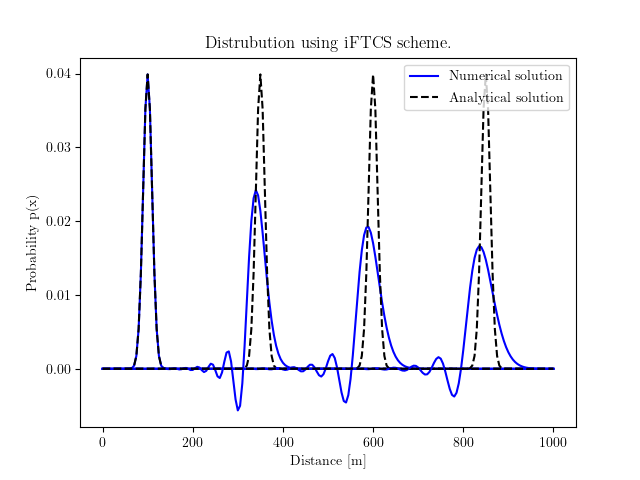
\includegraphics[width=0.9\textwidth]{../code/2d.png}
	\caption{Plot using the iFTCS scheme for the same t values as for figure \ref{fig:2c2}. We can see that whilst the iFTCS is unconditionally stable, our results are far off that of the analytical solution. We also so artifacts of the numerical methods, tailing the our curves.}
	\label{fig:2d}
\end{figure}
Whilst the iFTCS scheme is unconditionally stable\cite{bookA}, it does not mean that it would produce the best results. As we can see from figure \ref{fig:2d}, we are far off the analytical results. However from the iFTCS scheme, we can at least draw some conclusion, whilst rather poor, we can still have a better idea of where the woman will be at each time step. And knowing one thing or two about numerical methods, we can rule out the numerical artifacts and are left with a solution which have three peaks, at almost the same mean x-values as for the analytical solutions. Thus we are able to, with a fairly high accuracy, guesstimate where the woman will be.

\subsection{e)}
To simulate a more realistic case, we will consider a river with eddies. The eddies will cause the woman to remain stationary for some time, before probably keep moving with the river flow. This can be modeled as diffusion, as the probability of finding the woman at time t, would increase laterally, widening the range where we can find the woman. We will be using a diffusivity D = $0.5 m^2/s$.

We will start off by looking at this using the FTCS scheme, which is stable when we add diffusivity to the problem\cite{lev02}. The base equation for our problem now becomes
\begin{equation}
	\frac{\partial}{\partial t} p + u \frac{\partial}{\partial x}p = D\frac{\partial^2}{\partial x^2} p
\end{equation}
where $D$ is the diffusivity of the probability which we assume to be constant.
For the FTCS scheme from equation \ref{eq:disc} we get an additional term and our expression we now look as follows
\begin{align}
	\frac{p_i^{n+1}-p_i^n}{\Delta t} + u\frac{p_{i+1}^n - p_{i-1}^n}{2\Delta x} &= D\frac{p^n_{i+1} - 2p^n_i + p^n_{i-1}}{\Delta x^2}\\
	p_i^{n+1} &= -\frac{C_0}{2} \left(p_{i+1}^n - p_{i-1}^n\right) + 
	s\left(p^n_{i+1} - 2p^n_i + p^n_{i-1}\right) + p_i^n
\end{align}
where $C_0$ is defined as for the FTCS scheme \ref{eq:disc}, and $s = (D \Delta t)/\Delta x^2$. Collecting terms
\begin{equation}\label{eq:FTCSDiffu}
		p_i^{n+1} = \left(s - \frac{C_0}{2}\right)p_{i+1}^{n} 
		+ \left(1 - 2s\right)p_i^n 
		+ \left(s + \frac{C_0}{2}\right)p_{i-1}^n.
\end{equation}
From equation \ref{eq:FTCSDiffu} we can create our matrix $\mathbf{P}$ in the same way as for $\ref{mat:FTCS}$, thus being able to solve the following equation 
\begin{equation}
	p^{n+1} = \mathbf{P}p^n.
\end{equation}

\subsection{f)}
Adapting this problem to the same initial conditions as in c), we only need to make one adaption again, that is how we define the matrix $\mathbf{P}$. 
This can be done with the following function 
\lstinputlisting[firstline=32, lastline=45]{../code/2e.py}
From studying the relation between the advection transport rate and diffusive transport rate, we get what is called a P\'eclet number, which in this case is 10. As this number is greater than 1, we know that the advection dominates our equation. From this we should expect that we would see a greater transport down stream, than lateral spread of the probability function. 
The results of this we can see in figure \ref{fig:2e}, with numerical curves closely resemble those from d). 

Compared to what we found in c), using the FTCS scheme, we know have a stable solution, however this comes to no shock. As stated earlier, when we add a diffusive term to our advection equation the scheme becomes stable. What we can also note of importance, is that the analytical and numerical solution are very close in value, and we have no numerical artifacts in the plots that are visible. 

The analytical solution is given by 
\begin{equation}
	P(x,t) = \frac{1}{2\sqrt{\pi Dt}}\exp\left(-\frac{\left(x-ut\right)^2}{4Dt}\right).
\end{equation}
This stems from the same solution method as for the initial equation \ref{PDF_i}, where we use method of characteristics, and we assume that we have an initial point source, with a standard deviation. So our initial point source would be given by the Gaussian function \ref{PDF_i}. 
\begin{figure}
	\centering
	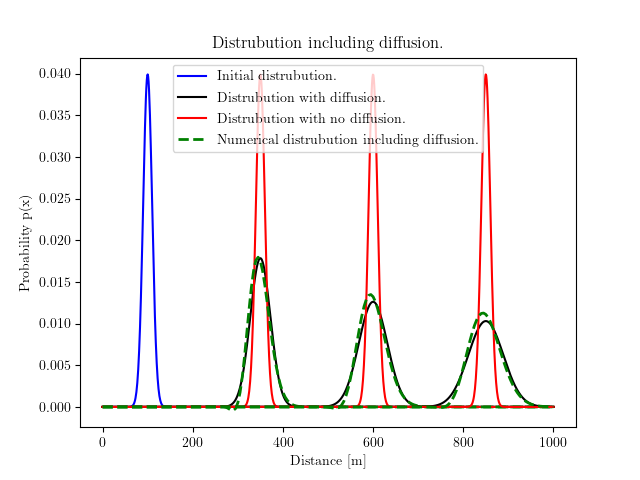
\includegraphics[width=0.9\textwidth]{../code/2e.png}
	\caption{Plot of analytical and numerical values found with diffusion. Included also is the analytical results from c). We have not included the numerical results from c), but we can see that the shape of our analytical curves closely resembles those from figure \ref{fig:2d}. So we have numerical diffusion in d).}
	\label{fig:2e}
\end{figure}

\subsection{g)}
Studying a case where we have non-constant diffusivity at a point $x$ downstream from where the woman fell into the water. At this point, the diffusivity follows the following equation $D(x) = D_0 + D_1x$, where $D_0 = 0.5m^2/s$. $D_1$ is chosen with the following criteria: \textit{Chose $D_1$ such that the advective effect due to the non-constant diffusivity exactly cancels the advection by the river velocity.}. 

We have that $D'(x) = D_1$. 
Starting of with the advection-diffusion equation we get the following 
\begin{align}
	\frac{\partial }{\partial t}p + u\frac{\partial}{\partial x} p &= \frac{\partial}{\partial x} \left(D\frac{\partial}{\partial x}p\right)\\
	&= \frac{\partial}{\partial x}D\frac{\partial}{\partial x} p + D\frac{\partial^2}{\partial x^2}p\\
	\frac{\partial}{\partial t}p + \frac{\partial}{\partial x}\left[u - D_1\right] &= D\frac{\partial^2}{\partial x^2}
\end{align}
From this we have that $u = D_1$, which gives $D_1 = 0.5$. 

Now having a new expression for the diffusivity, we want to see over what distance the diffusivity would double. From table \ref{table:1}, we see different values of x which gives a doubling in diffusivity. 
\begin{table}
	\centering
	\caption{n is the index of the values that results in a double of D(x), with their respective x and D(x) values.}
	\label{table:1}
	\begin{tabular}{|c|c|c|}
		\hline
		n &	$x_k$ & $D(x_k)$  \\ 
		\hline\hline
		0 & 0 & 0.5 \\  
		1 & 1 & 1 \\
		2 & 3 & 2 \\ 
		3 & 7 & 4 \\  
		4 & 15 & 8 \\ 
		5 & 31 & 16 \\
		\hline		
	\end{tabular}
\end{table}
From this we have that 
\begin{align}
	2*D(x_{k+1}) &= D(x_k)\\
	\frac{1}{2} + \frac{1}{2}x_{k+1} &= 1 + x_k\\
	\frac{1}{2}x_{k+1} &= \frac{1}{2}+x_k\\
	x_{k+1} &= 2x_k + 1\label{eq:rec}
\end{align}
Which gives us that the diffusivity doubles, following the recurrence relation given by equation \ref{eq:rec}. 

Writing a short python script as below
\lstinputlisting[]{../code/2g.py}

We can use polynomial fit to find a governing equation for our recurrence relation can be given by 
\begin{equation}
	0.99999411\exp(0.69323699x).
\end{equation}
This equation does not produce exact values, however it gives us the ability to find different values of x, for which the diffusivity would double from the previous value.

In short, we see the first doubling at x = 1m, and then the next at x = 3m, which we see from table \ref{table:1}.w
\bibliography{bibp3}
\bibliographystyle{plain}
\end{document}
